\documentclass{article} % For LaTeX2e
\usepackage{nips15submit_e,times}
\usepackage{hyperref}
\usepackage{url}
\usepackage{graphicx}
%\documentstyle[nips14submit_09,times,art10]{article} % For LaTeX 2.09


\title{Efficient Approximate PageRank 10605 15 Fall}


\author{
Jingyuan Liu\\
AndrewId: jingyual\\
\texttt{jingyual@andrew.cmu.edu} \\
}


\newcommand{\fix}{\marginpar{FIX}}
\newcommand{\new}{\marginpar{NEW}}


\nipsfinalcopy % Uncomment for camera-ready version


\begin{document}
\maketitle



\section{Question 1}
The probability that the k-th point is the last to be eaten is $\frac{1}{n}$.

\begin{equation}
p (k \ is \ the \ last \ to \ be \ eaten) = \frac{1}{n}
\end{equation}

Before k is eaten, we must first eat the k-1 or k+1. Consider the symmetry, we
can asuume that it is the k-1 that is eaten before k. The k is the last means
that the k+1 must be eaten already before k. This could happen if the random
walk passes cloclwise from k-1 to k+1 before eating k.

The probability of eats k-1 before k+1 is $\frac{1}{2}$, because the graph is
symmetric.  To conclude, we could see this result is reasonable. The overall
probability of any point be the last one:

\begin{equation}
\sum_k^n p(k \ is \ the \ last \ one) = 1
\end{equation}


\section{Question 2}
We could use several different criteria to evaluate a static-graph sampling
algorithms:

In-degree and out-degree distribution.

The distribution of sizes of weakly connected and strongly connected components.

Hot-plot: The number P (h) of reachable pairs of nodes at distance or less.

Hot-plot on the largest WCC.

The distribution of the first left singular vector of the graph adjacency matrix
versus the rank.

The distribution of singular values of the graph adjacency matrix versus the the
rank.

The distribution of the defined clustering coefficient.


\section{Question 3}
Place more outlinks from V would not change the PageRank score. Basically, place
more outlinks would not directly increase the inlinks, therefore, would not
bring direct increase. On the other hand, the self-reservered flow is not
changed by the outlink numbers. In conclusion, placing more outlinks would not
change the PageRank score.

Obtain more links to V would increase the PageRank score, since more links to
the V website, the PageRank score would increase as defined.

Split V into two Va and Vb without any links between them and copy all out
links would not change the PageRank for V. This is because there would not be
more links to the V. So the PageRank score would not change.

Sybil Attack would increase the PageRank score. Basically, using Sybil Attack
would add more inlinks to V. This would increase the PageRank score.


\section{Question 4}


\subsection{Question 4.1}
\begin{figure}[h]
\begin{center}
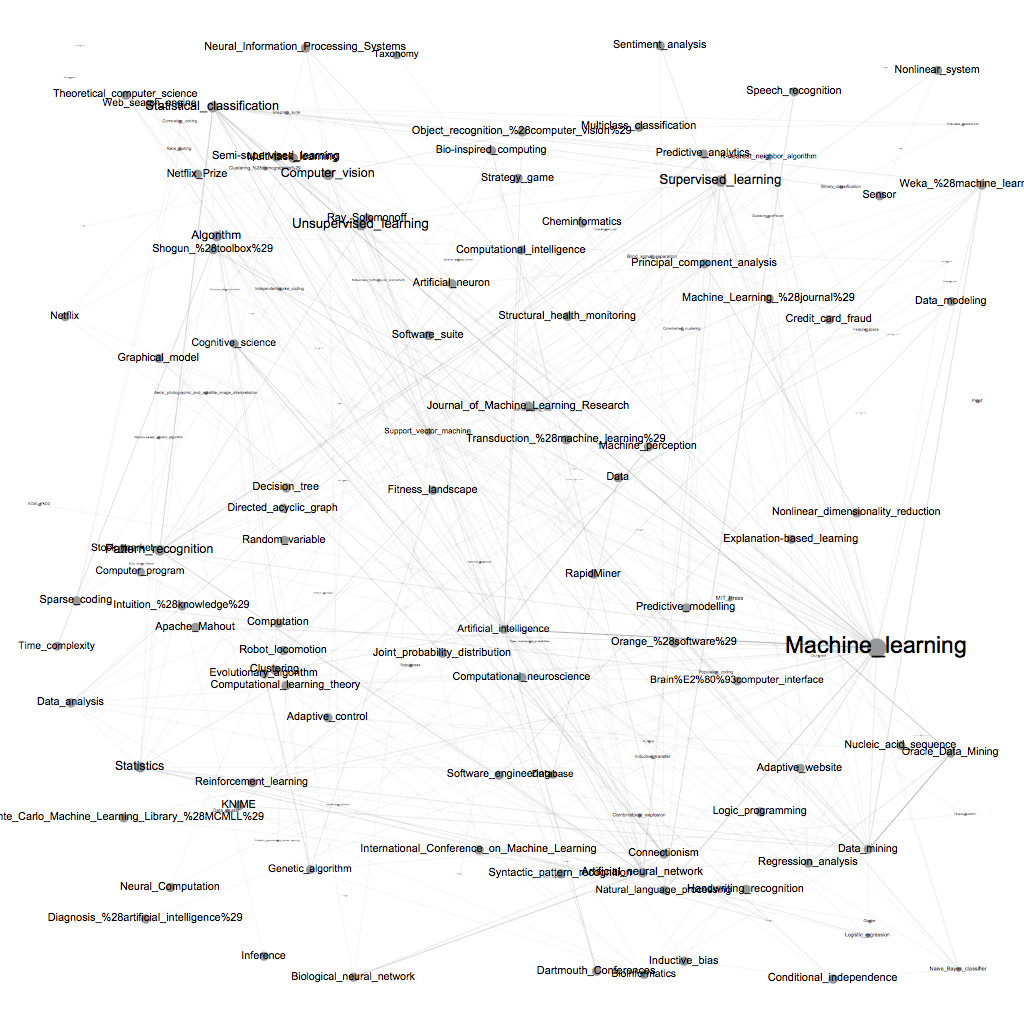
\includegraphics[width=10cm]{pic/result.png}
\end{center}
\caption{Gephi Graphics}
\end{figure}

\subsection{Question 4.2}
To cluster nodes into communities, we could use the ``clustering'' option in the
``windows'' panel. Or we could use the ``Modularity'' statistic to find
communities and assign ``cluster label'' to each community.

To find the authoritative nodes which are influencers in the network, we could
use the ``Ranking'',``Metrics'', and ``Filter'' options. We could select the
``Degree Range'' or some other metrics to filter those influencial points.


\section{Question 5}
I did not receive or give direct helps to other students.

\end{document}
